\documentclass{article}
\usepackage[left=0.5in,top=0.5in,right=0.5in,bottom=0.5in]{geometry}
\usepackage[english]{babel}
\usepackage[utf8]{inputenc}
\usepackage[table]{xcolor}
\usepackage{amssymb,amsmath,amsthm}
\usepackage{changepage,threeparttable}
\usepackage{booktabs,multirow}
\usepackage{graphicx}
\usepackage{soul}
\graphicspath{{./images/}}
\def\F#1{\(#1\)}
\title{Lab 8: The RC Filter}
\author{Philip Kim}
\date{\today}
\begin{document}
\maketitle
\vspace*{-1cm}
\begin{table}[!htp]\centering
  \begin{tabular}{|c|c|c|c|c|c|c|c|c|}\hline
    \multicolumn{9}{|c|}{\textbf{Table 1: High-Pass Filter}} \\\hline
    \F{f_{gen}}&\F{f_{osc}}&\F{C}&\F{R}&\F{V_{RC}}&\F{V_{R}}&\F{V/DIV~for~V_R}&\F{\left|H_{exp}\right|}&\F{\left|H_{the}\right|}\\\hline
    10kHz&10.010kHz&0.22\(\mu{F}\)&100\F{\Omega}&1.90V&1.74V&1V&0.8969&0.8105\\\hline
    5kHz&5.133kHz&0.22\(\mu{F}\)&100\F{\Omega}&1.98V&1.33V&1V&0.6717&0.5787\\\hline
    2kHz&2.222kHz&0.22\(\mu{F}\)&100\F{\Omega}&2.14V&0.77V&1V&0.3598&0.2936\\\hline
    1kHz&1.025kHz&0.22\(\mu{F}\)&100\F{\Omega}&2.10V&0.40V&1V&0.1905&0.1403\\\hline
    15kHz&15.143kHz&0.22\(\mu{F}\)&100\F{\Omega}&1.78V&1.90V&1V&0.9368&0.9023\\\hline
    20kHz&20.029kHz&0.22\(\mu{F}\)&100\F{\Omega}&1.86V&1.78V&1V&0.9570&0.9405\\\hline
    30kHz&30.024kHz&0.22\(\mu{F}\)&100\F{\Omega}&1.82V&1.78V&1V&0.9780&0.9722\\\hline
    40kHz&40.029kHz&0.22\(\mu{F}\)&100\F{\Omega}&1.74V&1.70V&1V&0.9770&0.9841\\\hline
  \end{tabular}
\end{table}
\begin{center}
  \subsection*{High-Pass Filter Setup}
  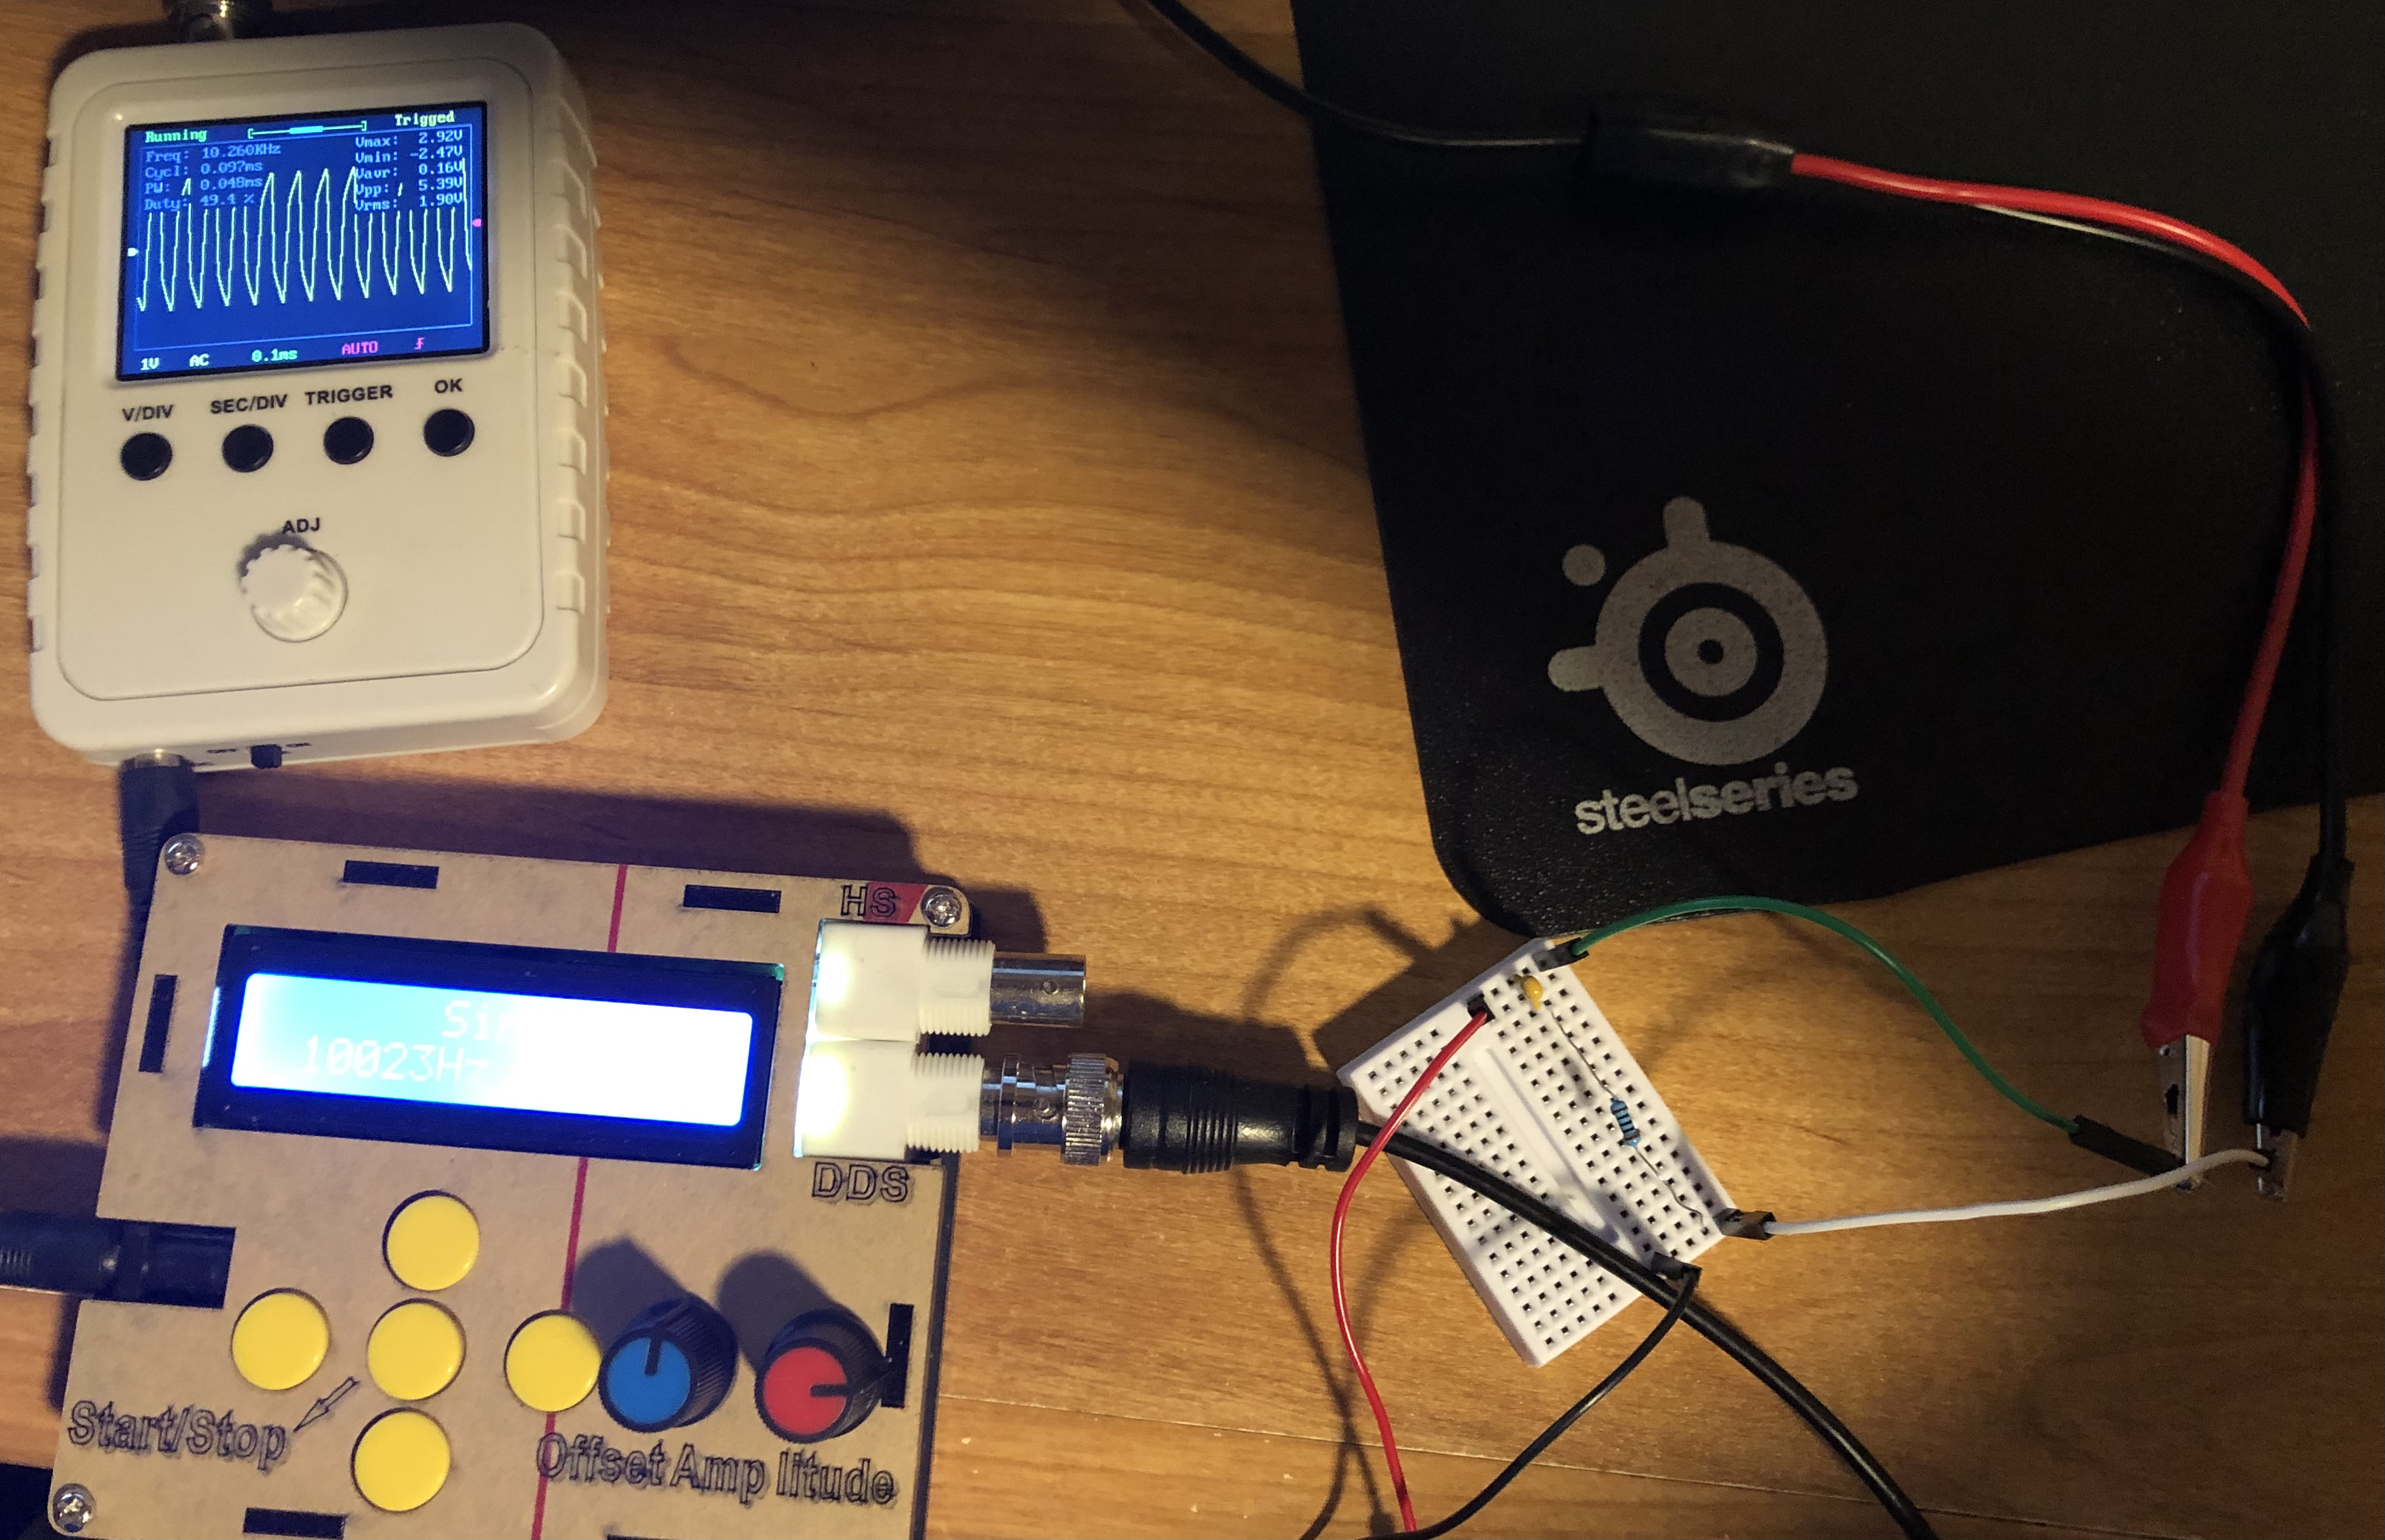
\includegraphics[scale=0.066]{Vrc.jpeg}
  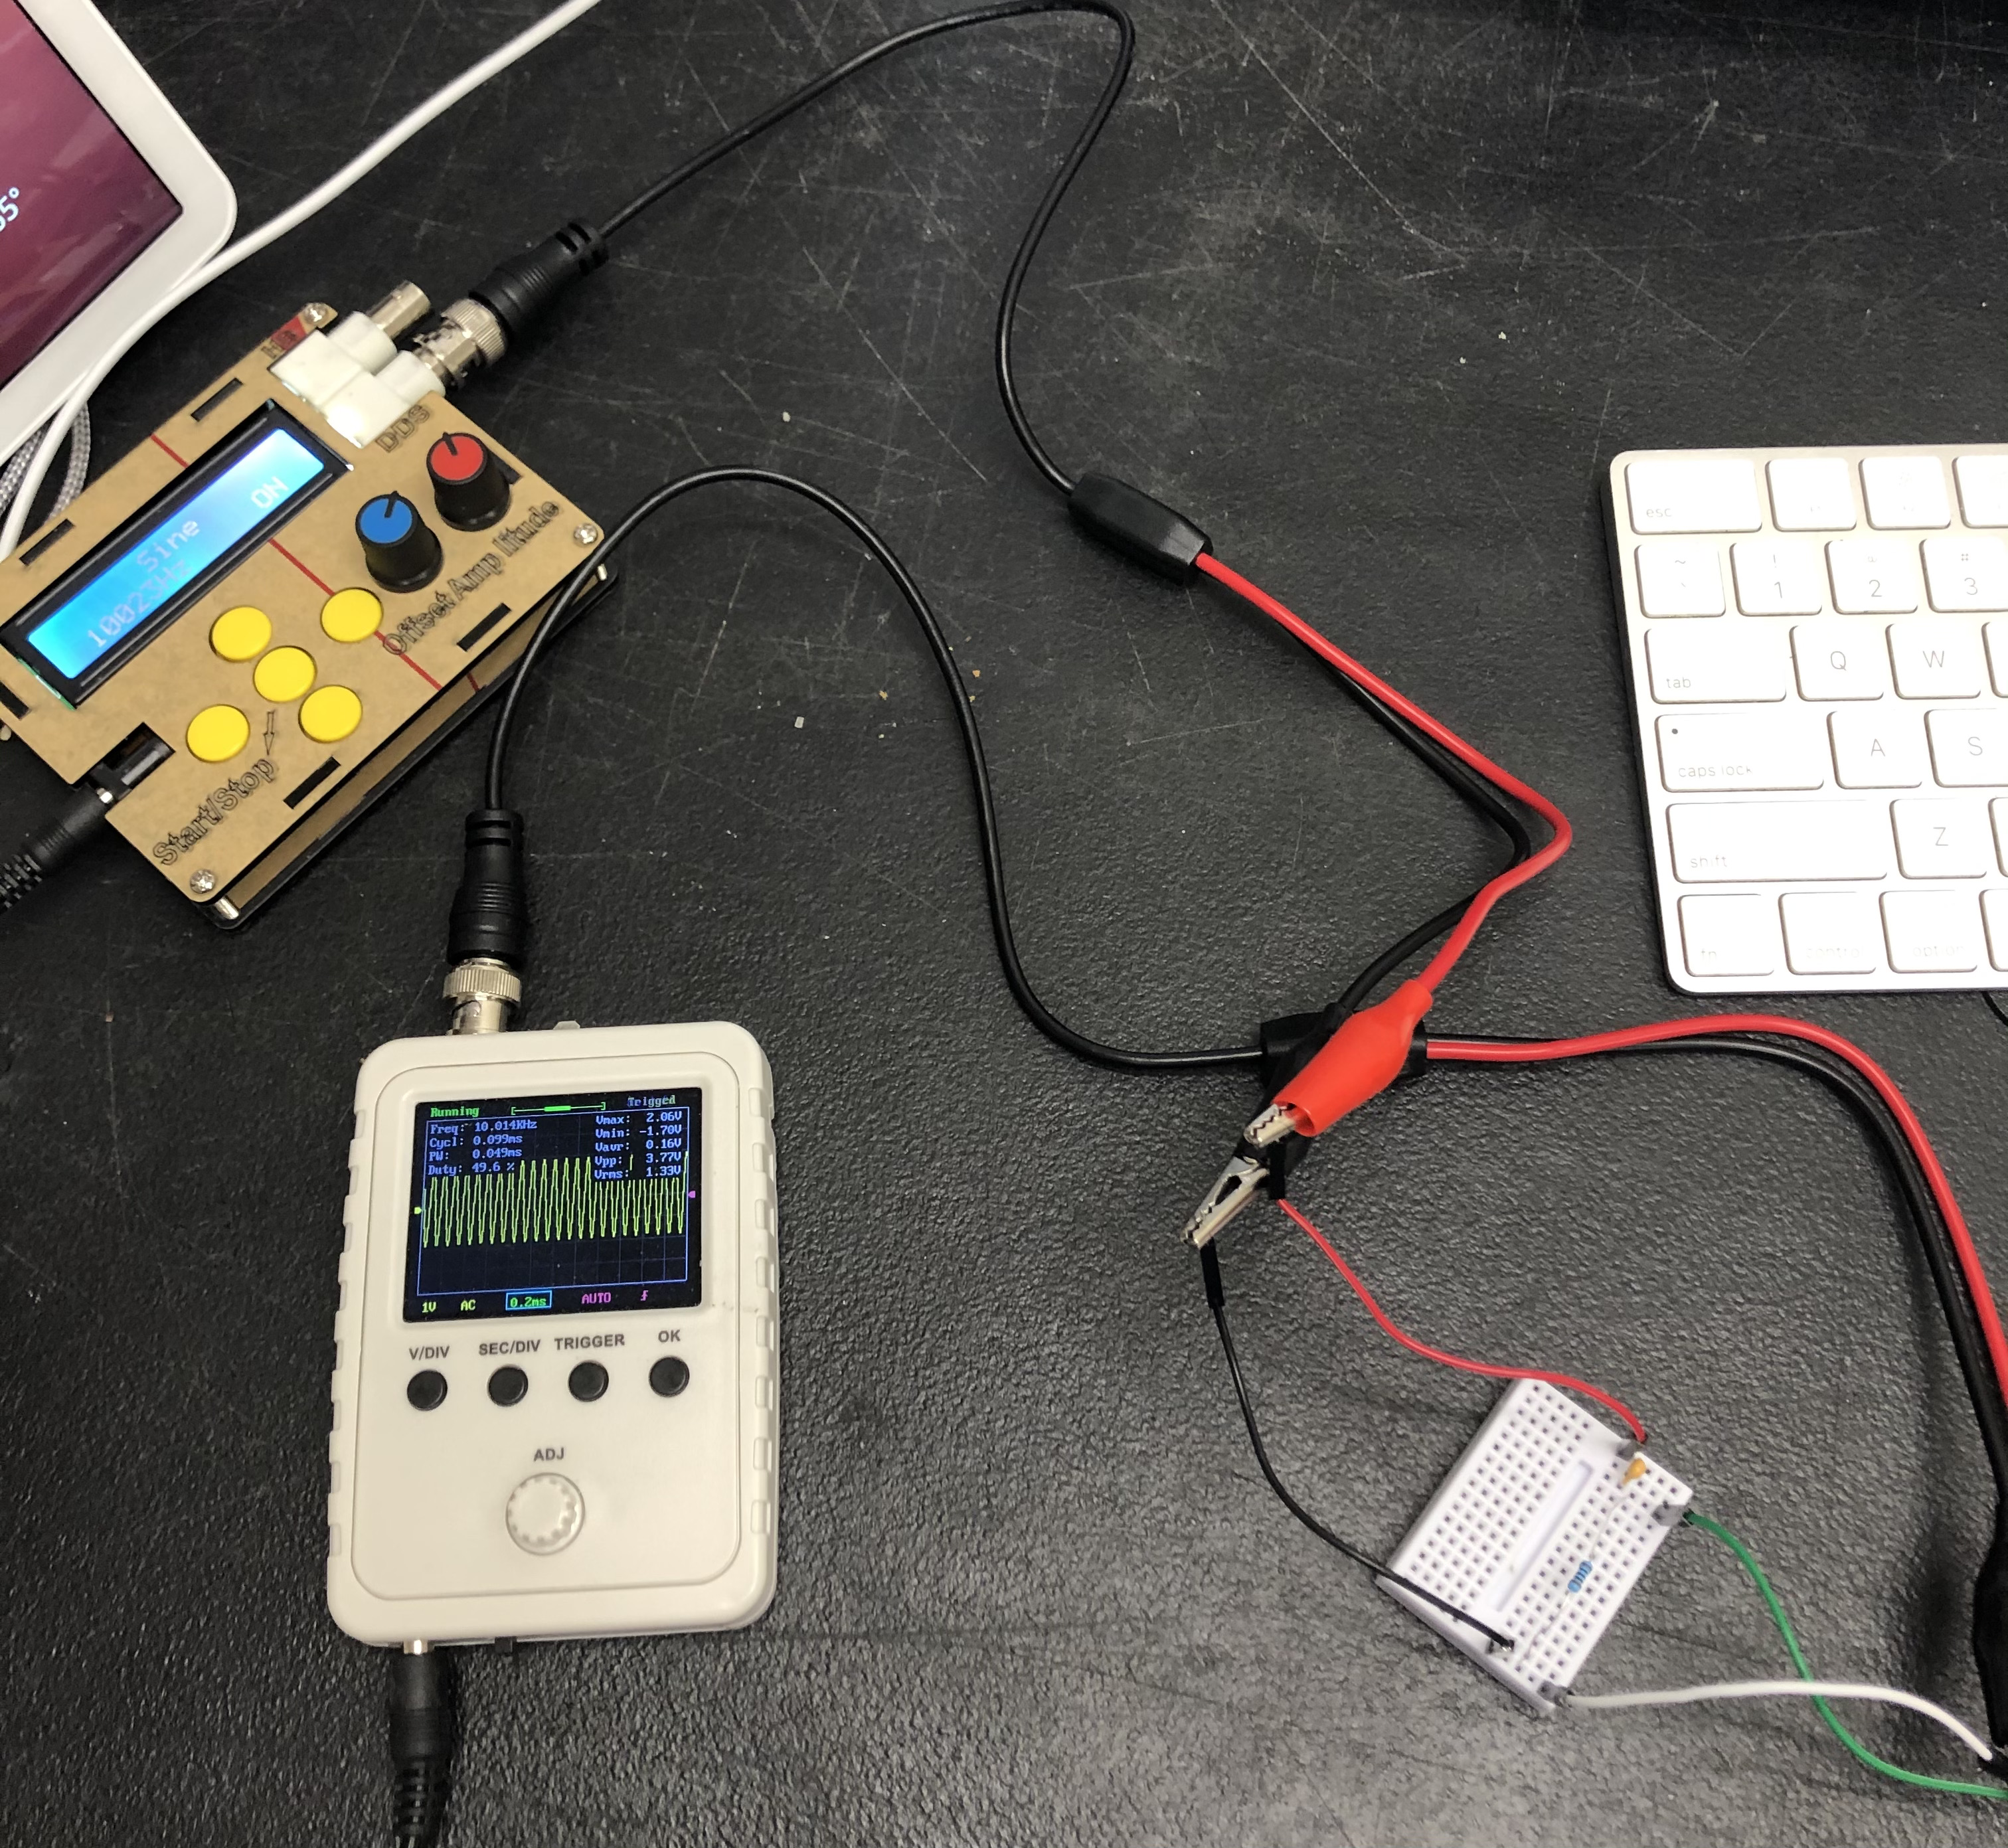
\includegraphics[scale=0.06]{Vr.jpeg}
\end{center}
\begin{center}
  \subsection*{High-Pass Filter Graph}
  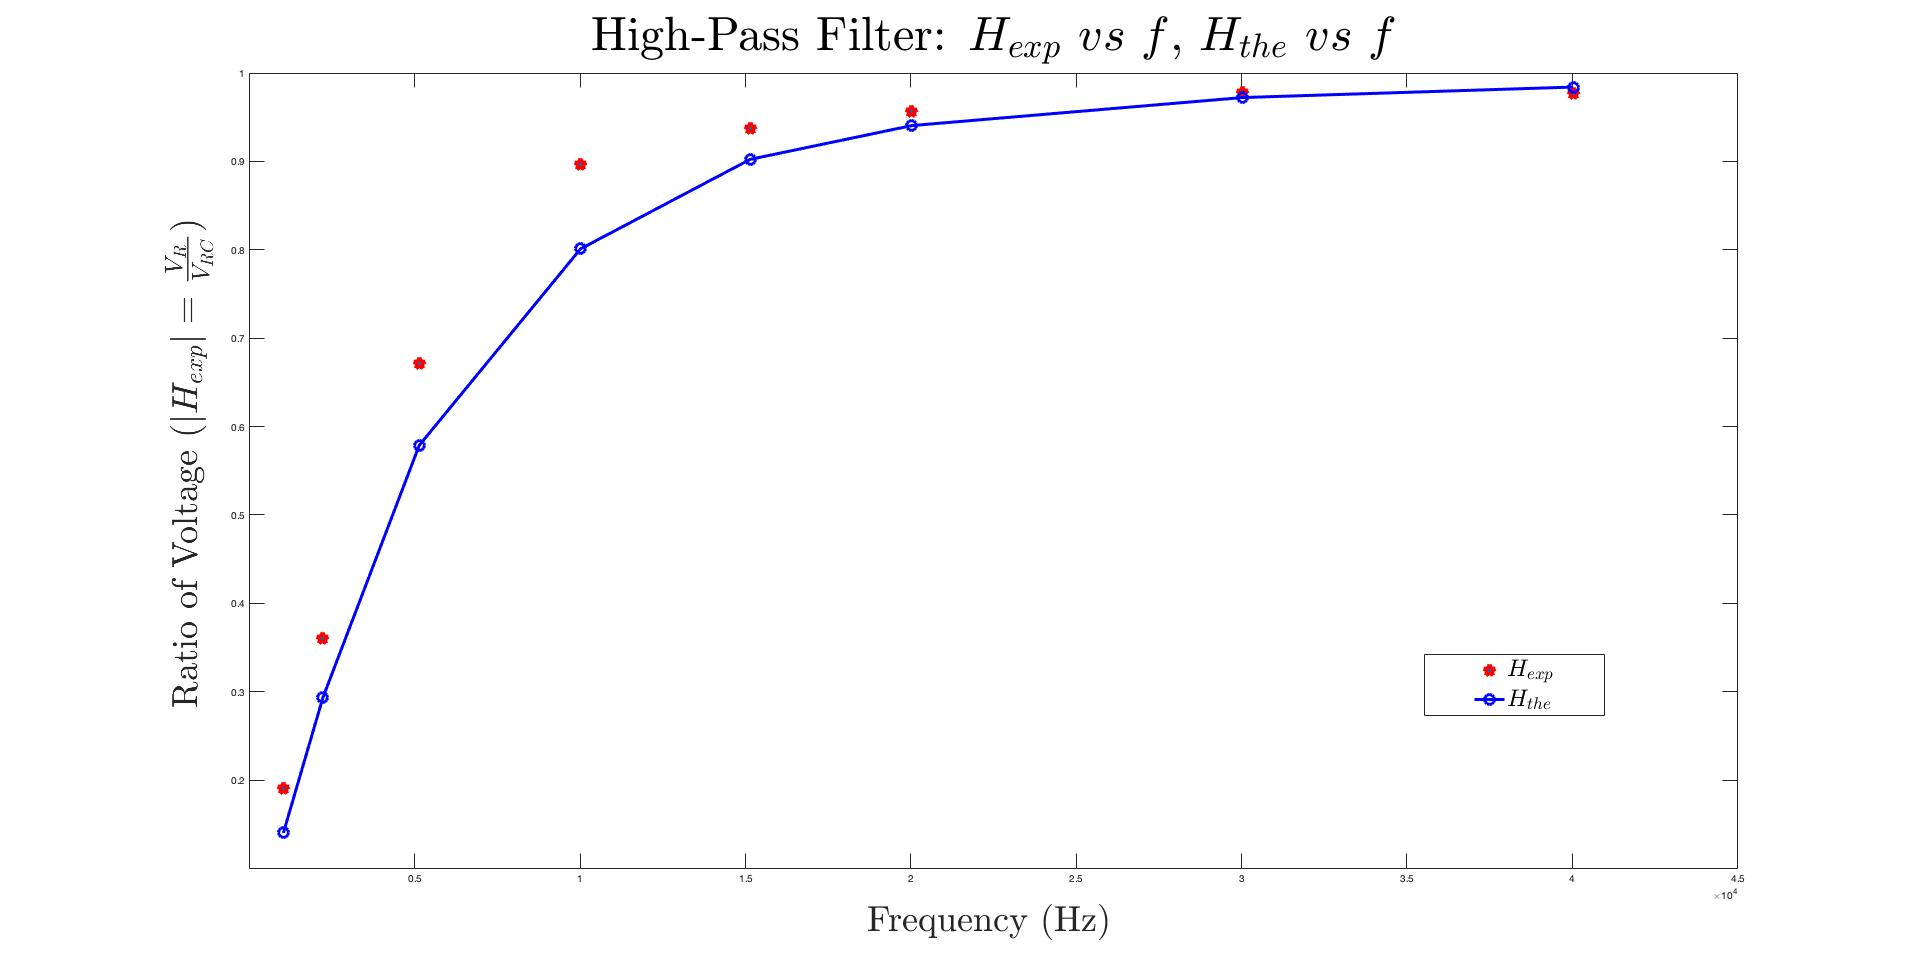
\includegraphics[scale=0.2]{graph1.jpg}
\end{center}
\newpage
\begin{table}[!htp]\centering
  \begin{tabular}{|c|c|c|c|c|c|c|c|c|}\hline
    \multicolumn{9}{|c|}{\textbf{Table 2: Low-Pass Filter}} \\\hline
    \F{f_{gen}}&\F{f_{osc}}&\F{C}&\F{R}&\F{V_{RC}}&\F{V_{C}}&\F{V/DIV~for~V_C}&\F{\left|H_{exp}\right|}&\F{\left|H_{the}\right|}\\\hline
    10kHz&10.010kHz&0.22\(\mu{F}\)&100\F{\Omega}&1.94V&1.09V&1V&0.5619&0.5857\\\hline
    5kHz&5.133kHz&0.22\(\mu{F}\)&100\F{\Omega}&1.94V&1.33V&1V&0.6856&0.8156\\\hline
    2kHz&2.222kHz&0.22\(\mu{F}\)&100\F{\Omega}&1.98V&1.70V&1V&0.8586&0.9559\\\hline
    1kHz& 1.138kHz&0.22\(\mu{F}\)&100\F{\Omega}&1.94V&1.86V&1V&0.9588&0.9879\\\hline
    15kHz&15.143kHz&0.22\(\mu{F}\)&100\F{\Omega}&1.86V&0.64V&1V&0.3441&0.4311\\\hline
    20kHz&20.029kHz&0.22\(\mu{F}\)&100\F{\Omega}&1.82V&0.52V&1V&0.2857&0.3397\\\hline
    30kHz&30.019kHz&0.22\(\mu{F}\)&100\F{\Omega}&1.70V&0.36V&1V&0.2218&0.2343\\\hline
    40kHz&40.029kHz&0.22\(\mu{F}\)&100\F{\Omega}&1.66V&0.28V&1V&0.1687&0.1778\\\hline
  \end{tabular}
\end{table}
\begin{center}
  \subsection*{Low-Pass Filter Setup}
  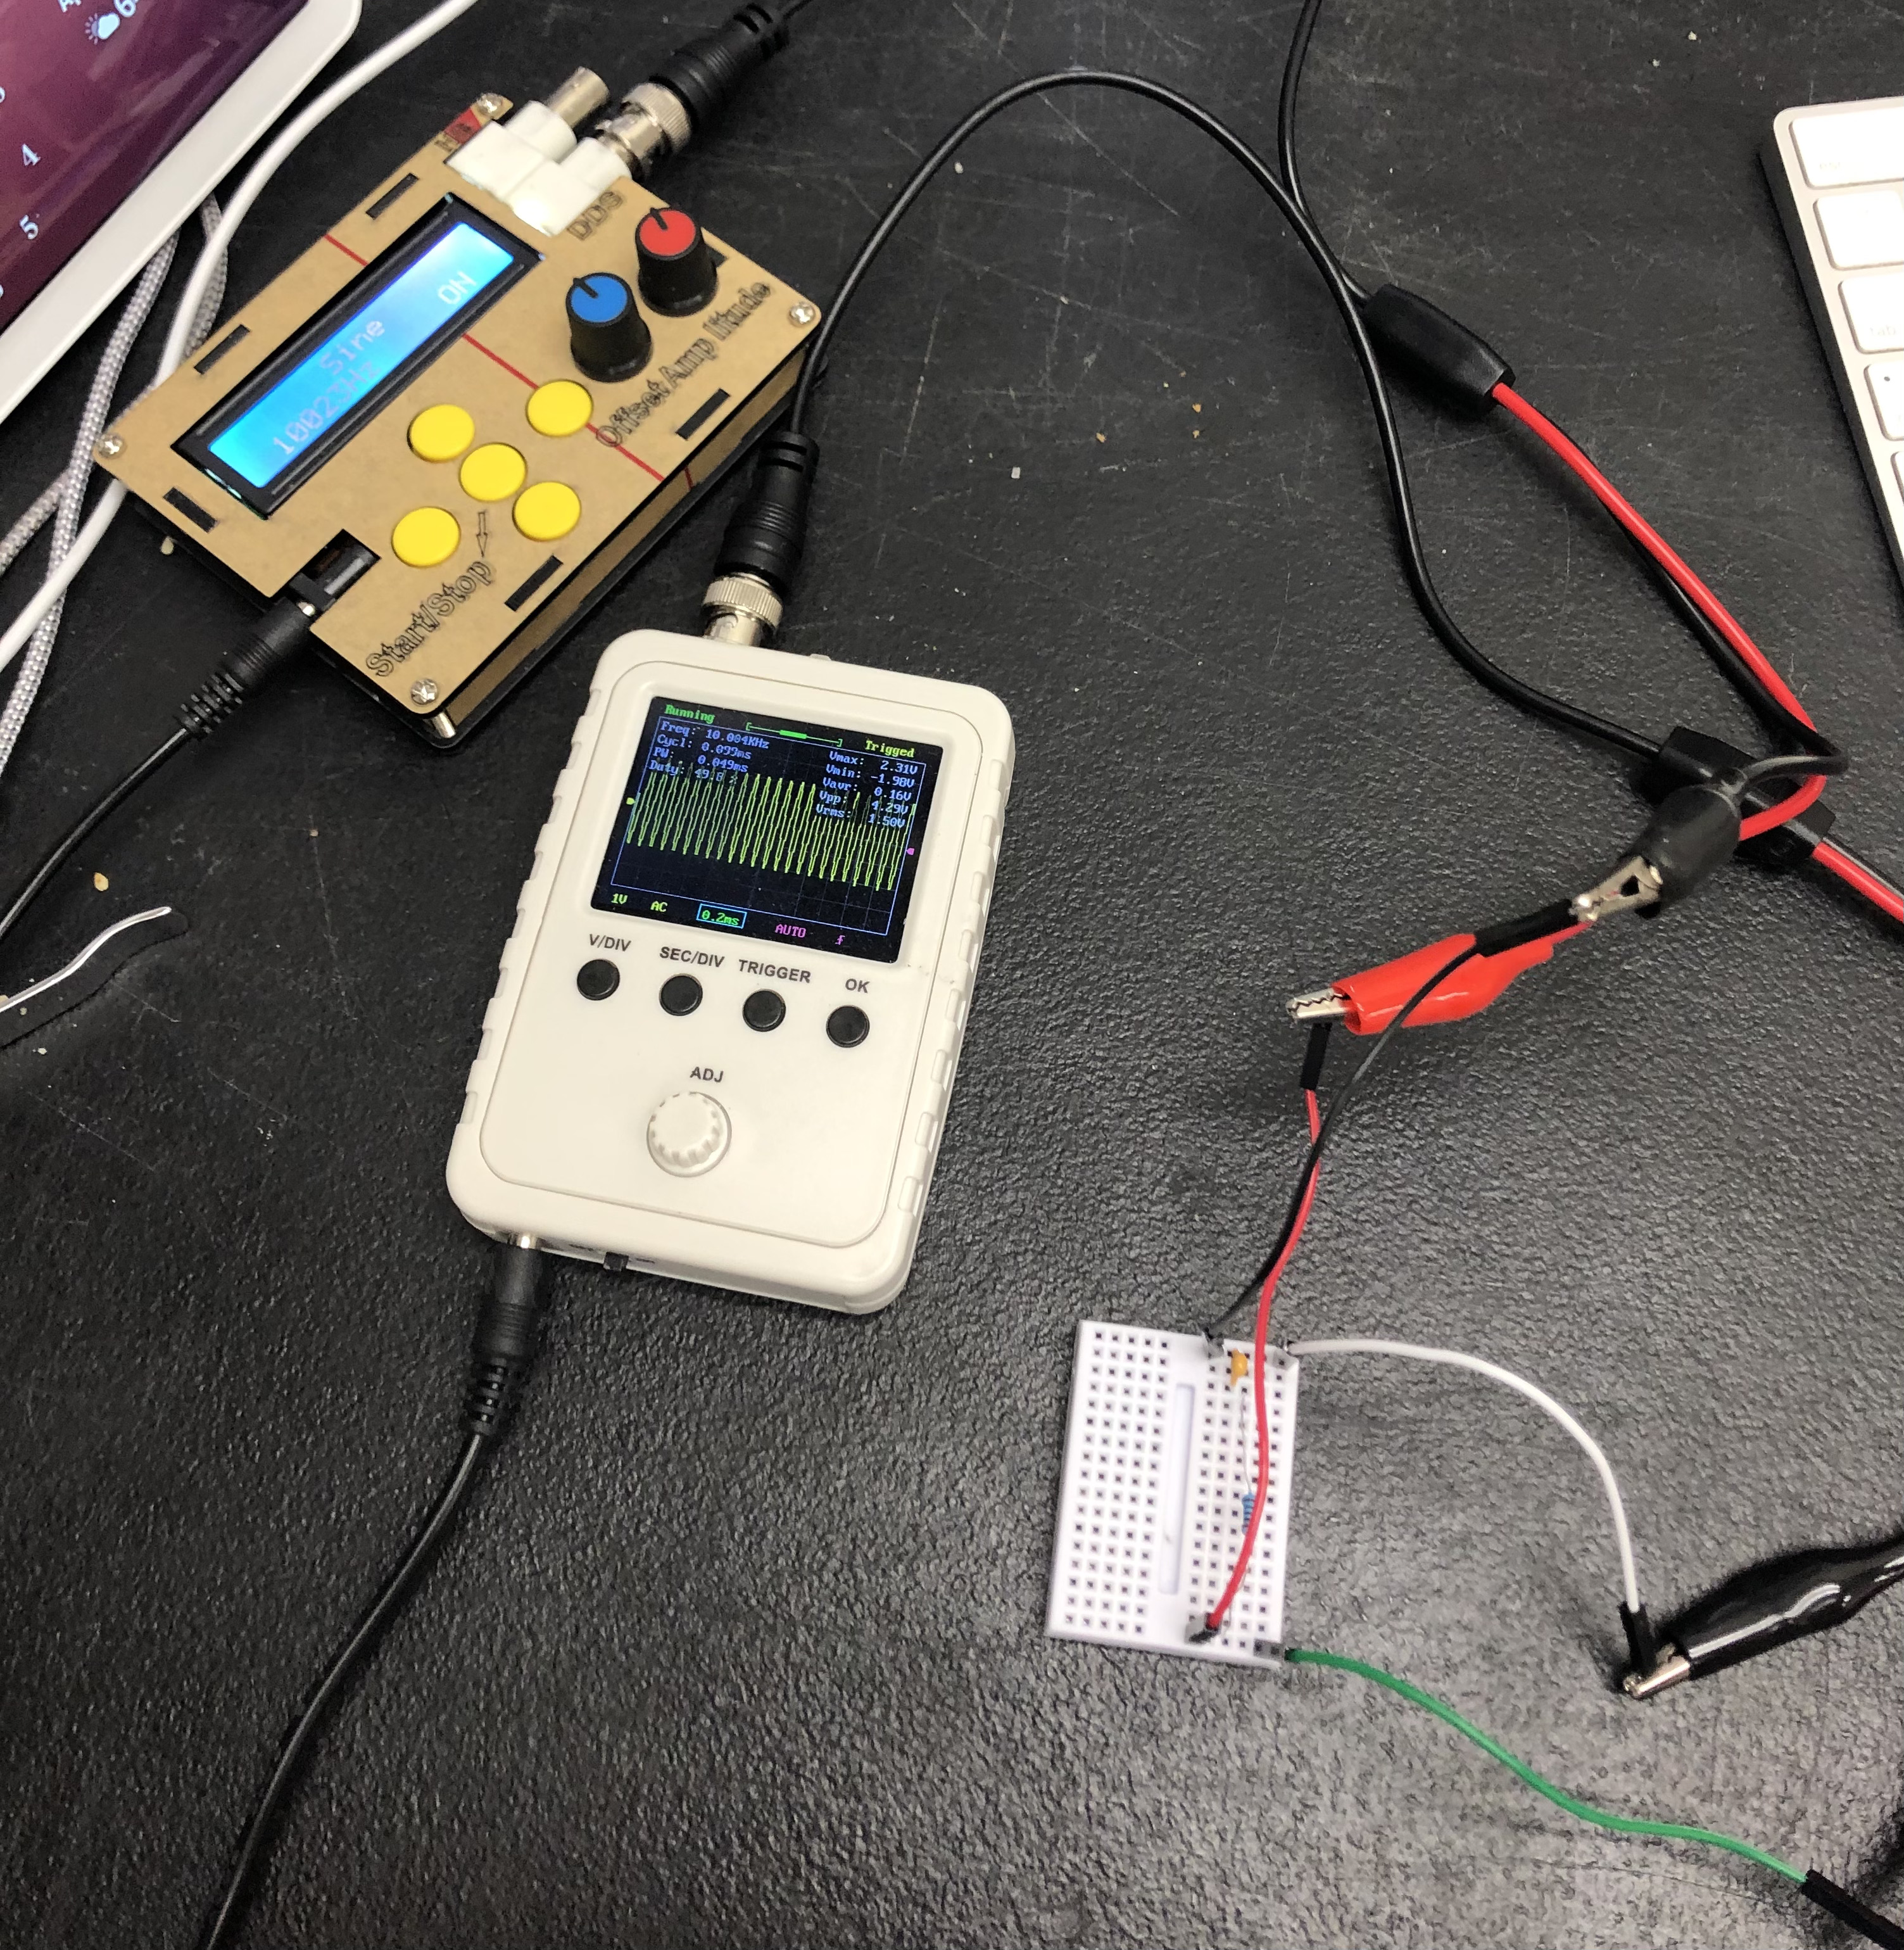
\includegraphics[scale=0.064]{Vcr.jpeg}
  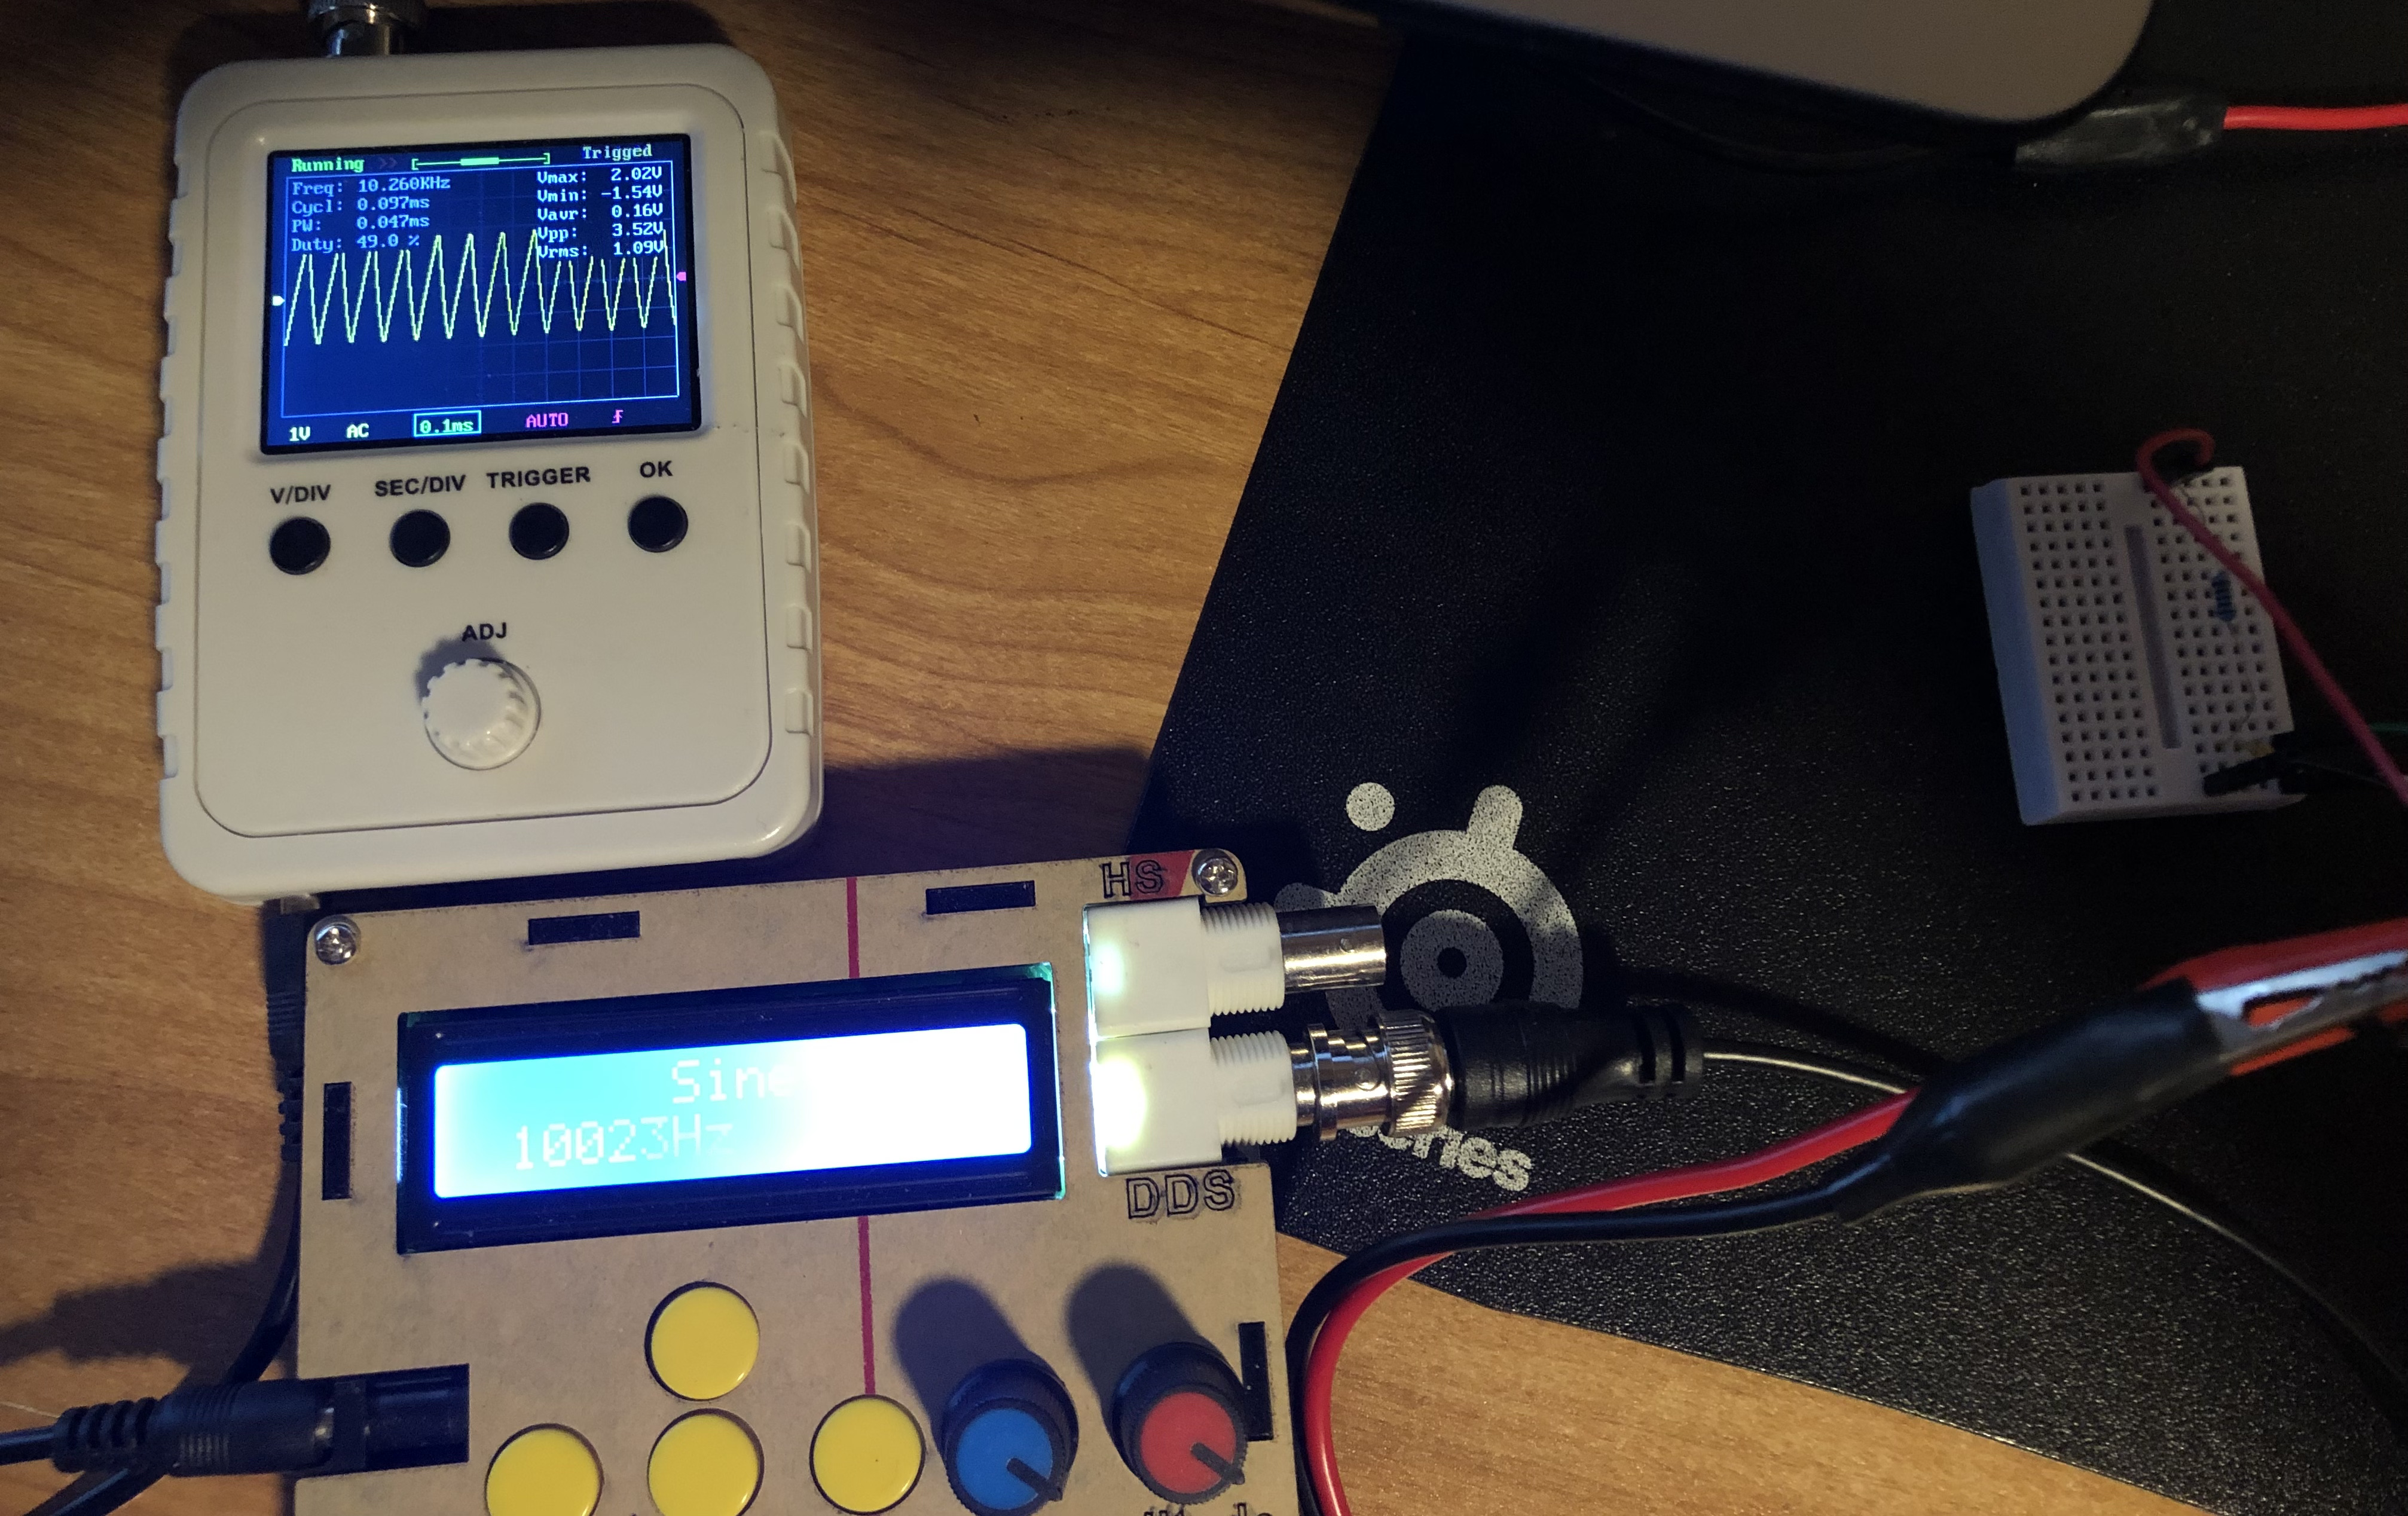
\includegraphics[scale=0.06]{Vc.jpeg}
\end{center}

\begin{center}
  \subsection*{Low-Pass Filter Graph}
  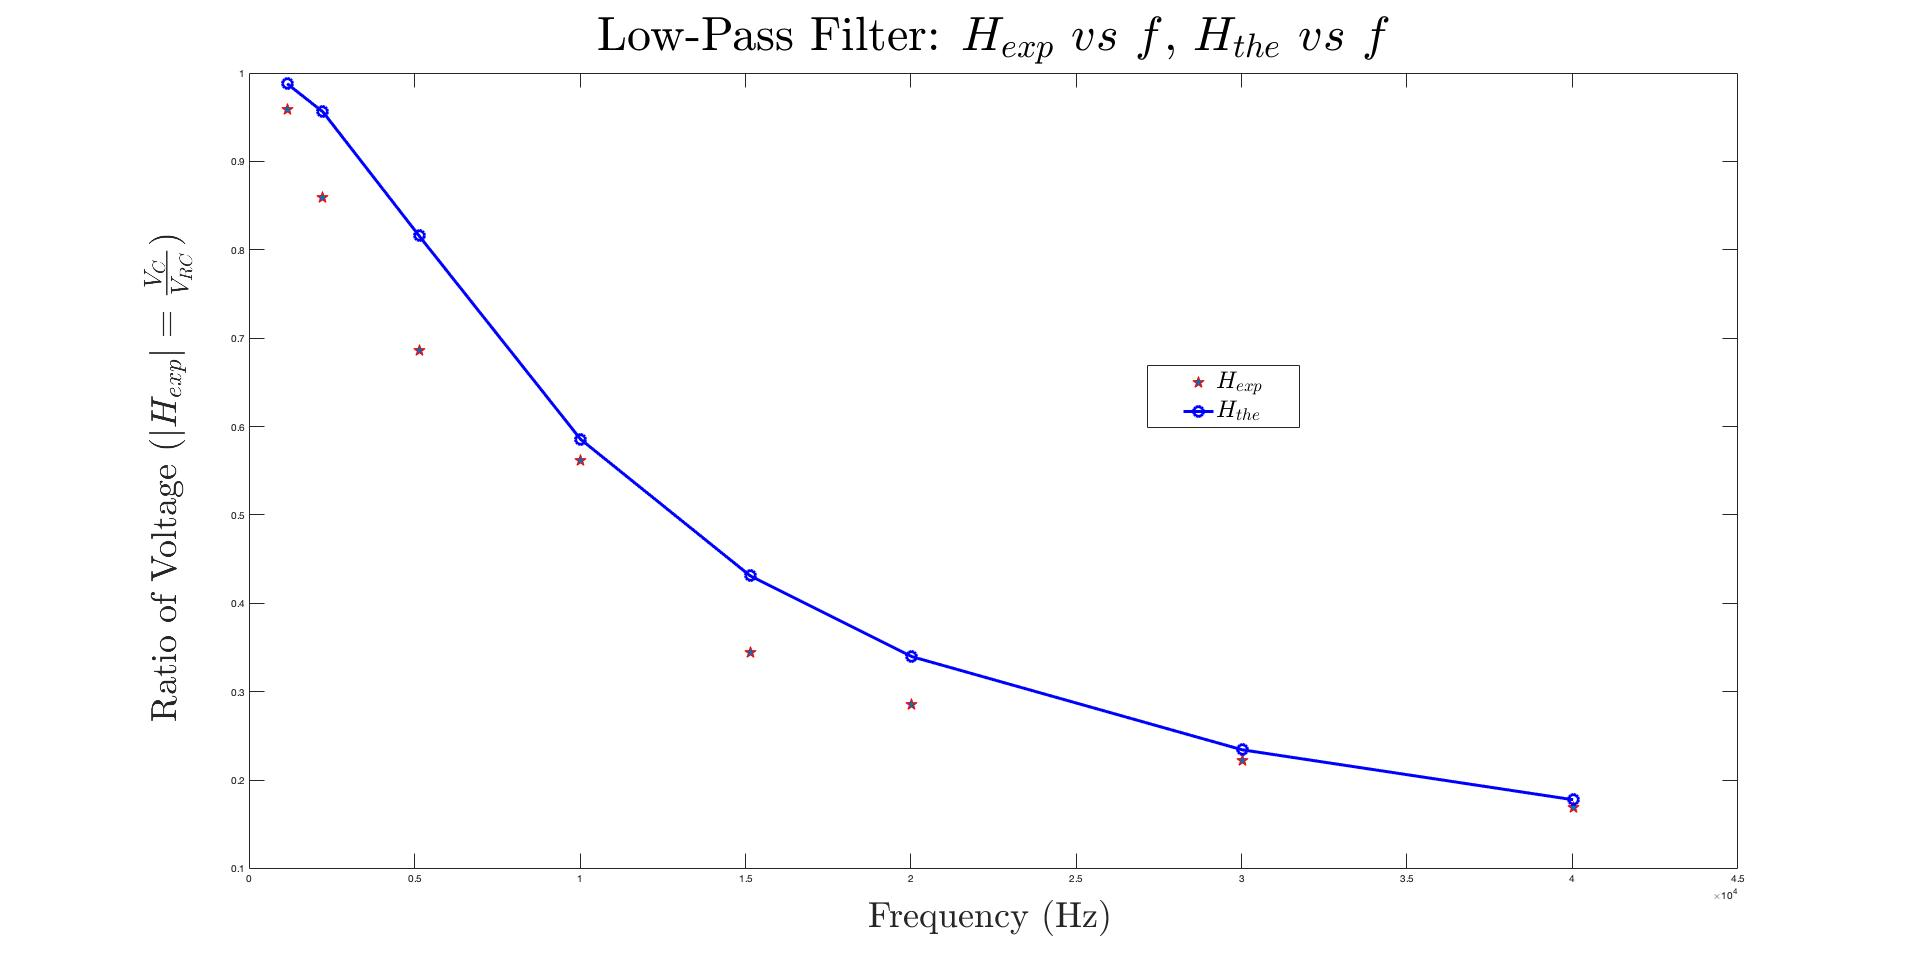
\includegraphics[scale=0.2]{graph2.jpg}
\end{center}

\begin{center}
  \begin{enumerate}
    \item Compare the theoretically obtained curves with the experimentally determined curves and quantify any difference. What do you think this difference is due to?
    \begin{itemize}
      \item High-Pass Filter: \(H_{the}\) curve is below \(H_{exp}\) symbols because the high pass filter only allows high frequency signals from its cut-off frequency, \(f_C\) point and higher to infinity to pass through while blocking those any lower.
      \item Low-Pass Filter: \(H_{the}\) curve is above \(H_{exp}\) symbols because the low pass filter only allows low frequency signals from 0Hz to its cut-off frequency, \(f_C\) point to pass while blocking those any higher.
    \end{itemize}
  \end{enumerate}
\end{center}
\end{document}
